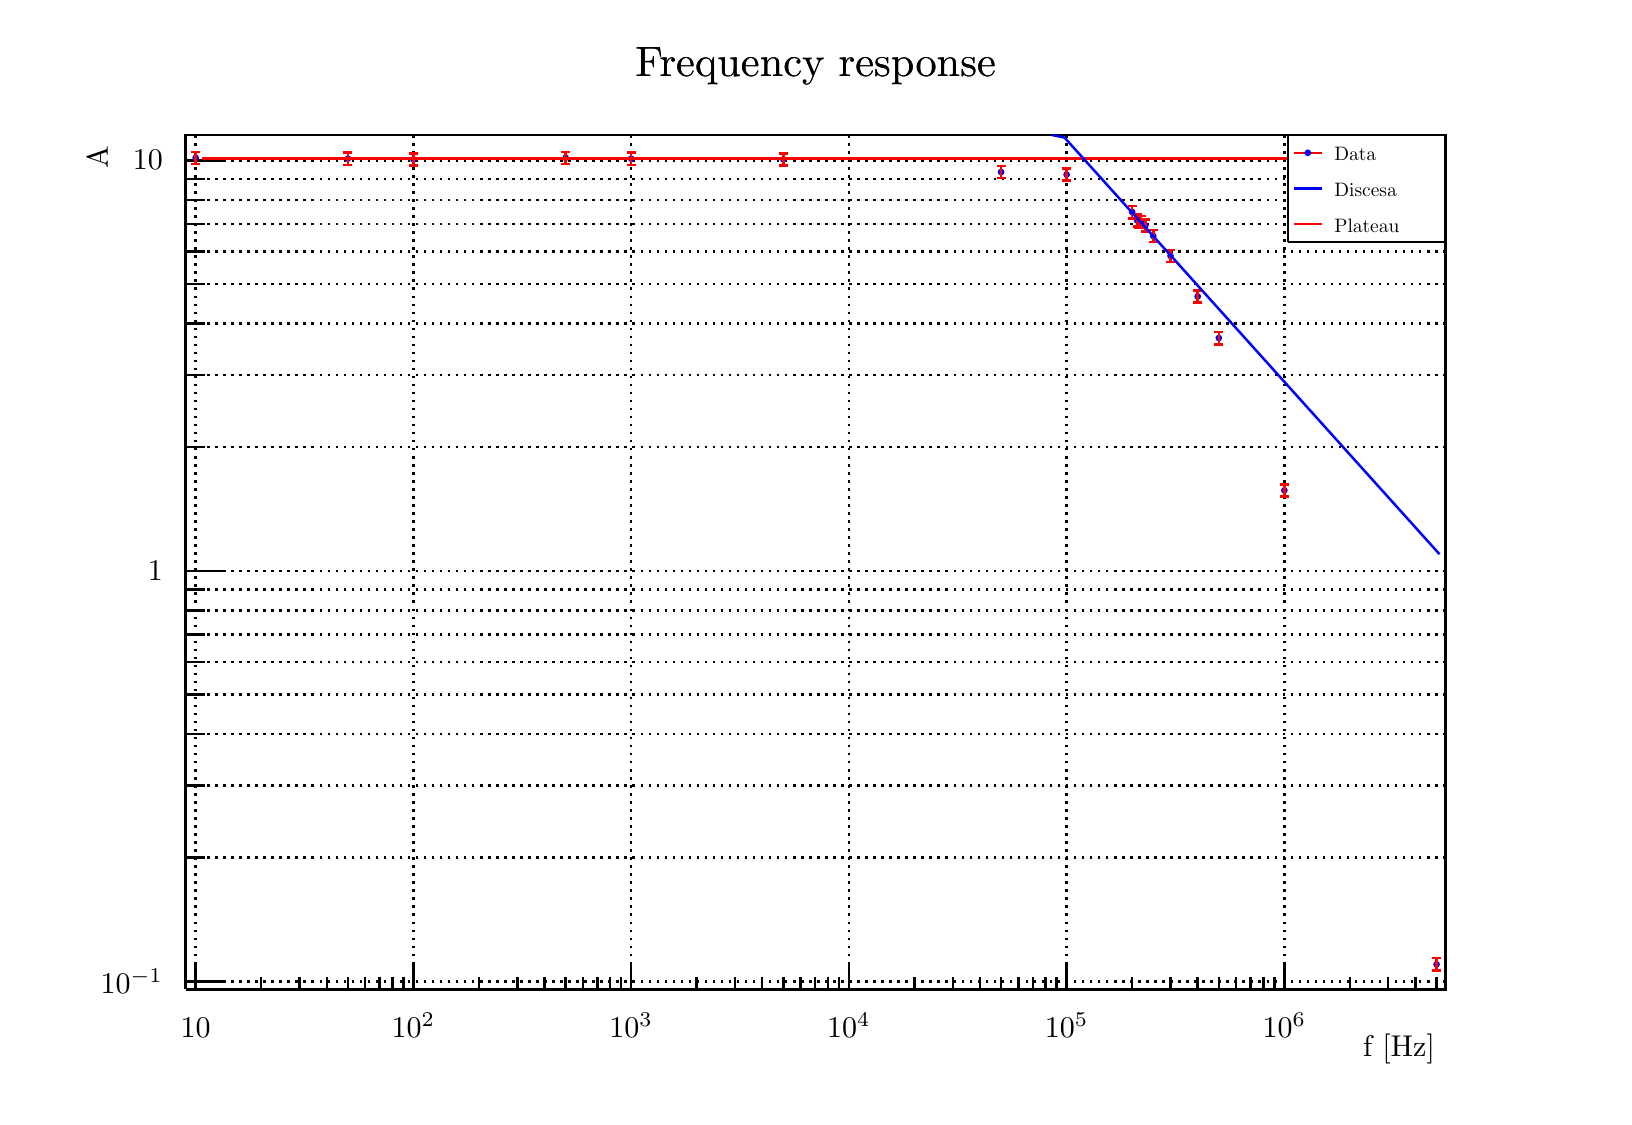
\begin{tikzpicture}
\pgfdeclareplotmark{cross} {
\pgfpathmoveto{\pgfpoint{-0.3\pgfplotmarksize}{\pgfplotmarksize}}
\pgfpathlineto{\pgfpoint{+0.3\pgfplotmarksize}{\pgfplotmarksize}}
\pgfpathlineto{\pgfpoint{+0.3\pgfplotmarksize}{0.3\pgfplotmarksize}}
\pgfpathlineto{\pgfpoint{+1\pgfplotmarksize}{0.3\pgfplotmarksize}}
\pgfpathlineto{\pgfpoint{+1\pgfplotmarksize}{-0.3\pgfplotmarksize}}
\pgfpathlineto{\pgfpoint{+0.3\pgfplotmarksize}{-0.3\pgfplotmarksize}}
\pgfpathlineto{\pgfpoint{+0.3\pgfplotmarksize}{-1.\pgfplotmarksize}}
\pgfpathlineto{\pgfpoint{-0.3\pgfplotmarksize}{-1.\pgfplotmarksize}}
\pgfpathlineto{\pgfpoint{-0.3\pgfplotmarksize}{-0.3\pgfplotmarksize}}
\pgfpathlineto{\pgfpoint{-1.\pgfplotmarksize}{-0.3\pgfplotmarksize}}
\pgfpathlineto{\pgfpoint{-1.\pgfplotmarksize}{0.3\pgfplotmarksize}}
\pgfpathlineto{\pgfpoint{-0.3\pgfplotmarksize}{0.3\pgfplotmarksize}}
\pgfpathclose
\pgfusepathqstroke
}
\pgfdeclareplotmark{cross*} {
\pgfpathmoveto{\pgfpoint{-0.3\pgfplotmarksize}{\pgfplotmarksize}}
\pgfpathlineto{\pgfpoint{+0.3\pgfplotmarksize}{\pgfplotmarksize}}
\pgfpathlineto{\pgfpoint{+0.3\pgfplotmarksize}{0.3\pgfplotmarksize}}
\pgfpathlineto{\pgfpoint{+1\pgfplotmarksize}{0.3\pgfplotmarksize}}
\pgfpathlineto{\pgfpoint{+1\pgfplotmarksize}{-0.3\pgfplotmarksize}}
\pgfpathlineto{\pgfpoint{+0.3\pgfplotmarksize}{-0.3\pgfplotmarksize}}
\pgfpathlineto{\pgfpoint{+0.3\pgfplotmarksize}{-1.\pgfplotmarksize}}
\pgfpathlineto{\pgfpoint{-0.3\pgfplotmarksize}{-1.\pgfplotmarksize}}
\pgfpathlineto{\pgfpoint{-0.3\pgfplotmarksize}{-0.3\pgfplotmarksize}}
\pgfpathlineto{\pgfpoint{-1.\pgfplotmarksize}{-0.3\pgfplotmarksize}}
\pgfpathlineto{\pgfpoint{-1.\pgfplotmarksize}{0.3\pgfplotmarksize}}
\pgfpathlineto{\pgfpoint{-0.3\pgfplotmarksize}{0.3\pgfplotmarksize}}
\pgfpathclose
\pgfusepathqfillstroke
}
\pgfdeclareplotmark{newstar} {
\pgfpathmoveto{\pgfqpoint{0pt}{\pgfplotmarksize}}
\pgfpathlineto{\pgfqpointpolar{44}{0.5\pgfplotmarksize}}
\pgfpathlineto{\pgfqpointpolar{18}{\pgfplotmarksize}}
\pgfpathlineto{\pgfqpointpolar{-20}{0.5\pgfplotmarksize}}
\pgfpathlineto{\pgfqpointpolar{-54}{\pgfplotmarksize}}
\pgfpathlineto{\pgfqpointpolar{-90}{0.5\pgfplotmarksize}}
\pgfpathlineto{\pgfqpointpolar{234}{\pgfplotmarksize}}
\pgfpathlineto{\pgfqpointpolar{198}{0.5\pgfplotmarksize}}
\pgfpathlineto{\pgfqpointpolar{162}{\pgfplotmarksize}}
\pgfpathlineto{\pgfqpointpolar{134}{0.5\pgfplotmarksize}}
\pgfpathclose
\pgfusepathqstroke
}
\pgfdeclareplotmark{newstar*} {
\pgfpathmoveto{\pgfqpoint{0pt}{\pgfplotmarksize}}
\pgfpathlineto{\pgfqpointpolar{44}{0.5\pgfplotmarksize}}
\pgfpathlineto{\pgfqpointpolar{18}{\pgfplotmarksize}}
\pgfpathlineto{\pgfqpointpolar{-20}{0.5\pgfplotmarksize}}
\pgfpathlineto{\pgfqpointpolar{-54}{\pgfplotmarksize}}
\pgfpathlineto{\pgfqpointpolar{-90}{0.5\pgfplotmarksize}}
\pgfpathlineto{\pgfqpointpolar{234}{\pgfplotmarksize}}
\pgfpathlineto{\pgfqpointpolar{198}{0.5\pgfplotmarksize}}
\pgfpathlineto{\pgfqpointpolar{162}{\pgfplotmarksize}}
\pgfpathlineto{\pgfqpointpolar{134}{0.5\pgfplotmarksize}}
\pgfpathclose
\pgfusepathqfillstroke
}
\definecolor{c}{rgb}{1,1,1};
\draw [color=c, fill=c] (0,0) rectangle (20,13.5632);
\draw [color=c, fill=c] (2,1.35632) rectangle (18,12.2069);
\definecolor{c}{rgb}{0,0,0};
\draw [c,line width=0.9] (2,1.35632) -- (2,12.2069) -- (18,12.2069) -- (18,1.35632) -- (2,1.35632);
\draw [c,line width=0.9] (2,1.35632) -- (18,1.35632);
\draw [c,dotted,line width=0.9] (2.12653,12.2069) -- (2.12653,1.35632);
\draw [c,dotted,line width=0.9] (4.89177,12.2069) -- (4.89177,1.35632);
\draw [c,dotted,line width=0.9] (7.657,12.2069) -- (7.657,1.35632);
\draw [c,dotted,line width=0.9] (10.4222,12.2069) -- (10.4222,1.35632);
\draw [c,dotted,line width=0.9] (13.1875,12.2069) -- (13.1875,1.35632);
\draw [c,dotted,line width=0.9] (15.9527,12.2069) -- (15.9527,1.35632);
\draw [c,line width=0.9] (2,1.35632) -- (2,12.2069);
\draw [c,dotted,line width=0.9] (18,1.4593) -- (2,1.4593);
\draw [c,dotted,line width=0.9] (18,3.02864) -- (2,3.02864);
\draw [c,dotted,line width=0.9] (18,3.94665) -- (2,3.94665);
\draw [c,dotted,line width=0.9] (18,4.59799) -- (2,4.59799);
\draw [c,dotted,line width=0.9] (18,5.1032) -- (2,5.1032);
\draw [c,dotted,line width=0.9] (18,5.516) -- (2,5.516);
\draw [c,dotted,line width=0.9] (18,5.86501) -- (2,5.86501);
\draw [c,dotted,line width=0.9] (18,6.16733) -- (2,6.16733);
\draw [c,dotted,line width=0.9] (18,6.434) -- (2,6.434);
\draw [c,dotted,line width=0.9] (18,6.67255) -- (2,6.67255);
\draw [c,dotted,line width=0.9] (18,8.24189) -- (2,8.24189);
\draw [c,dotted,line width=0.9] (18,9.1599) -- (2,9.1599);
\draw [c,dotted,line width=0.9] (18,9.81124) -- (2,9.81124);
\draw [c,dotted,line width=0.9] (18,10.3165) -- (2,10.3165);
\draw [c,dotted,line width=0.9] (18,10.7292) -- (2,10.7292);
\draw [c,dotted,line width=0.9] (18,11.0783) -- (2,11.0783);
\draw [c,dotted,line width=0.9] (18,11.3806) -- (2,11.3806);
\draw [c,dotted,line width=0.9] (18,11.6472) -- (2,11.6472);
\draw [c,dotted,line width=0.9] (18,11.8858) -- (2,11.8858);
\draw [c,line width=0.9] (2,1.35632) -- (18,1.35632);
\draw [anchor= east] (18,0.596782) node[scale=1.08496, color=c, rotate=0]{f [Hz]};
\draw [c,line width=0.9] (2.12653,1.68184) -- (2.12653,1.35632);
\draw [anchor=base] (2.12653,0.742586) node[scale=1.08496, color=c, rotate=0]{10};
\draw [c,line width=0.9] (2.95895,1.51908) -- (2.95895,1.35632);
\draw [c,line width=0.9] (3.44588,1.51908) -- (3.44588,1.35632);
\draw [c,line width=0.9] (3.79137,1.51908) -- (3.79137,1.35632);
\draw [c,line width=0.9] (4.05935,1.51908) -- (4.05935,1.35632);
\draw [c,line width=0.9] (4.2783,1.51908) -- (4.2783,1.35632);
\draw [c,line width=0.9] (4.46343,1.51908) -- (4.46343,1.35632);
\draw [c,line width=0.9] (4.62379,1.51908) -- (4.62379,1.35632);
\draw [c,line width=0.9] (4.76524,1.51908) -- (4.76524,1.35632);
\draw [c,line width=0.9] (4.89177,1.68184) -- (4.89177,1.35632);
\draw [anchor=base] (4.89177,0.742586) node[scale=1.08496, color=c, rotate=0]{$10^{2}$};
\draw [c,line width=0.9] (5.72419,1.51908) -- (5.72419,1.35632);
\draw [c,line width=0.9] (6.21112,1.51908) -- (6.21112,1.35632);
\draw [c,line width=0.9] (6.55661,1.51908) -- (6.55661,1.35632);
\draw [c,line width=0.9] (6.82458,1.51908) -- (6.82458,1.35632);
\draw [c,line width=0.9] (7.04354,1.51908) -- (7.04354,1.35632);
\draw [c,line width=0.9] (7.22866,1.51908) -- (7.22866,1.35632);
\draw [c,line width=0.9] (7.38903,1.51908) -- (7.38903,1.35632);
\draw [c,line width=0.9] (7.53047,1.51908) -- (7.53047,1.35632);
\draw [c,line width=0.9] (7.657,1.68184) -- (7.657,1.35632);
\draw [anchor=base] (7.657,0.742586) node[scale=1.08496, color=c, rotate=0]{$10^{3}$};
\draw [c,line width=0.9] (8.48942,1.51908) -- (8.48942,1.35632);
\draw [c,line width=0.9] (8.97636,1.51908) -- (8.97636,1.35632);
\draw [c,line width=0.9] (9.32184,1.51908) -- (9.32184,1.35632);
\draw [c,line width=0.9] (9.58982,1.51908) -- (9.58982,1.35632);
\draw [c,line width=0.9] (9.80878,1.51908) -- (9.80878,1.35632);
\draw [c,line width=0.9] (9.9939,1.51908) -- (9.9939,1.35632);
\draw [c,line width=0.9] (10.1543,1.51908) -- (10.1543,1.35632);
\draw [c,line width=0.9] (10.2957,1.51908) -- (10.2957,1.35632);
\draw [c,line width=0.9] (10.4222,1.68184) -- (10.4222,1.35632);
\draw [anchor=base] (10.4222,0.742586) node[scale=1.08496, color=c, rotate=0]{$10^{4}$};
\draw [c,line width=0.9] (11.2547,1.51908) -- (11.2547,1.35632);
\draw [c,line width=0.9] (11.7416,1.51908) -- (11.7416,1.35632);
\draw [c,line width=0.9] (12.0871,1.51908) -- (12.0871,1.35632);
\draw [c,line width=0.9] (12.3551,1.51908) -- (12.3551,1.35632);
\draw [c,line width=0.9] (12.574,1.51908) -- (12.574,1.35632);
\draw [c,line width=0.9] (12.7591,1.51908) -- (12.7591,1.35632);
\draw [c,line width=0.9] (12.9195,1.51908) -- (12.9195,1.35632);
\draw [c,line width=0.9] (13.061,1.51908) -- (13.061,1.35632);
\draw [c,line width=0.9] (13.1875,1.68184) -- (13.1875,1.35632);
\draw [anchor=base] (13.1875,0.742586) node[scale=1.08496, color=c, rotate=0]{$10^{5}$};
\draw [c,line width=0.9] (14.0199,1.51908) -- (14.0199,1.35632);
\draw [c,line width=0.9] (14.5068,1.51908) -- (14.5068,1.35632);
\draw [c,line width=0.9] (14.8523,1.51908) -- (14.8523,1.35632);
\draw [c,line width=0.9] (15.1203,1.51908) -- (15.1203,1.35632);
\draw [c,line width=0.9] (15.3393,1.51908) -- (15.3393,1.35632);
\draw [c,line width=0.9] (15.5244,1.51908) -- (15.5244,1.35632);
\draw [c,line width=0.9] (15.6847,1.51908) -- (15.6847,1.35632);
\draw [c,line width=0.9] (15.8262,1.51908) -- (15.8262,1.35632);
\draw [c,line width=0.9] (15.9527,1.68184) -- (15.9527,1.35632);
\draw [anchor=base] (15.9527,0.742586) node[scale=1.08496, color=c, rotate=0]{$10^{6}$};
\draw [c,line width=0.9] (16.7851,1.51908) -- (16.7851,1.35632);
\draw [c,line width=0.9] (17.2721,1.51908) -- (17.2721,1.35632);
\draw [c,line width=0.9] (17.6176,1.51908) -- (17.6176,1.35632);
\draw [c,line width=0.9] (17.8855,1.51908) -- (17.8855,1.35632);
\draw [c,line width=0.9] (2,1.35632) -- (2,12.2069);
\draw [anchor= east] (0.88,12.2069) node[scale=1.08496, color=c, rotate=90]{A};
\draw [c,line width=0.9] (2.48,1.4593) -- (2,1.4593);
\draw [anchor= east] (1.844,1.4593) node[scale=1.08496, color=c, rotate=0]{$10^{-1}$};
\draw [c,line width=0.9] (2.24,3.02864) -- (2,3.02864);
\draw [c,line width=0.9] (2.24,3.94665) -- (2,3.94665);
\draw [c,line width=0.9] (2.24,4.59799) -- (2,4.59799);
\draw [c,line width=0.9] (2.24,5.1032) -- (2,5.1032);
\draw [c,line width=0.9] (2.24,5.516) -- (2,5.516);
\draw [c,line width=0.9] (2.24,5.86501) -- (2,5.86501);
\draw [c,line width=0.9] (2.24,6.16733) -- (2,6.16733);
\draw [c,line width=0.9] (2.24,6.434) -- (2,6.434);
\draw [c,line width=0.9] (2.48,6.67255) -- (2,6.67255);
\draw [anchor= east] (1.844,6.67255) node[scale=1.08496, color=c, rotate=0]{1};
\draw [c,line width=0.9] (2.24,8.24189) -- (2,8.24189);
\draw [c,line width=0.9] (2.24,9.1599) -- (2,9.1599);
\draw [c,line width=0.9] (2.24,9.81124) -- (2,9.81124);
\draw [c,line width=0.9] (2.24,10.3165) -- (2,10.3165);
\draw [c,line width=0.9] (2.24,10.7292) -- (2,10.7292);
\draw [c,line width=0.9] (2.24,11.0783) -- (2,11.0783);
\draw [c,line width=0.9] (2.24,11.3806) -- (2,11.3806);
\draw [c,line width=0.9] (2.24,11.6472) -- (2,11.6472);
\draw [c,line width=0.9] (2.48,11.8858) -- (2,11.8858);
\draw [anchor= east] (1.844,11.8858) node[scale=1.08496, color=c, rotate=0]{10};
\draw (10,13.0816) node[scale=1.5317, color=c, rotate=0]{Frequency response};
\definecolor{c}{rgb}{0,0,1};
\foreach \P in {(2.12653,11.9173), (4.05935,11.9061), (4.89177,11.8971), (6.82459,11.9173), (7.65701,11.9061), (9.58983,11.8971), (12.3551,11.736), (13.1875,11.7044), (14.0199,11.2284), (14.0842,11.1231), (14.1068,11.1072), (14.1344,11.1072),
 (14.1877,11.0588), (14.2879,10.9244), (14.5068,10.6719), (14.8523,10.157), (15.1203,9.6286), (15.9527,7.69382), (17.8855,1.67509)}{\draw[mark options={color=c,fill=c},mark size=1.681682pt,mark=*,mark size=1pt] plot coordinates {\P};}
\definecolor{c}{rgb}{1,0,0};
\draw [c,line width=0.9] (2.12653,11.9173) -- (2.12653,11.9932);
\draw [c,line width=0.9] (2.06906,11.9932) -- (2.184,11.9932);
\draw [c,line width=0.9] (2.12653,11.9173) -- (2.12653,11.8387);
\draw [c,line width=0.9] (2.06906,11.8387) -- (2.184,11.8387);
\draw [c,line width=0.9] (4.05935,11.9061) -- (4.05935,11.9821);
\draw [c,line width=0.9] (4.00188,11.9821) -- (4.11682,11.9821);
\draw [c,line width=0.9] (4.05935,11.9061) -- (4.05935,11.8275);
\draw [c,line width=0.9] (4.00188,11.8275) -- (4.11682,11.8275);
\draw [c,line width=0.9] (4.89177,11.8971) -- (4.89177,11.9731);
\draw [c,line width=0.9] (4.8343,11.9731) -- (4.94924,11.9731);
\draw [c,line width=0.9] (4.89177,11.8971) -- (4.89177,11.8184);
\draw [c,line width=0.9] (4.8343,11.8184) -- (4.94924,11.8184);
\draw [c,line width=0.9] (6.82459,11.9173) -- (6.82459,11.9932);
\draw [c,line width=0.9] (6.76712,11.9932) -- (6.88206,11.9932);
\draw [c,line width=0.9] (6.82459,11.9173) -- (6.82459,11.8387);
\draw [c,line width=0.9] (6.76712,11.8387) -- (6.88206,11.8387);
\draw [c,line width=0.9] (7.65701,11.9061) -- (7.65701,11.9821);
\draw [c,line width=0.9] (7.59954,11.9821) -- (7.71448,11.9821);
\draw [c,line width=0.9] (7.65701,11.9061) -- (7.65701,11.8275);
\draw [c,line width=0.9] (7.59954,11.8275) -- (7.71448,11.8275);
\draw [c,line width=0.9] (9.58983,11.8971) -- (9.58983,11.9731);
\draw [c,line width=0.9] (9.53235,11.9731) -- (9.6473,11.9731);
\draw [c,line width=0.9] (9.58983,11.8971) -- (9.58983,11.8184);
\draw [c,line width=0.9] (9.53235,11.8184) -- (9.6473,11.8184);
\draw [c,line width=0.9] (12.3551,11.736) -- (12.3551,11.8102);
\draw [c,line width=0.9] (12.2976,11.8102) -- (12.4125,11.8102);
\draw [c,line width=0.9] (12.3551,11.736) -- (12.3551,11.6594);
\draw [c,line width=0.9] (12.2976,11.6594) -- (12.4125,11.6594);
\draw [c,line width=0.9] (13.1875,11.7044) -- (13.1875,11.7787);
\draw [c,line width=0.9] (13.13,11.7787) -- (13.245,11.7787);
\draw [c,line width=0.9] (13.1875,11.7044) -- (13.1875,11.6276);
\draw [c,line width=0.9] (13.13,11.6276) -- (13.245,11.6276);
\draw [c,line width=0.9] (14.0199,11.2284) -- (14.0199,11.3056);
\draw [c,line width=0.9] (13.9624,11.3056) -- (14.0774,11.3056);
\draw [c,line width=0.9] (14.0199,11.2284) -- (14.0199,11.1485);
\draw [c,line width=0.9] (13.9624,11.1485) -- (14.0774,11.1485);
\draw [c,line width=0.9] (14.0842,11.1231) -- (14.0842,11.1971);
\draw [c,line width=0.9] (14.0267,11.1971) -- (14.1417,11.1971);
\draw [c,line width=0.9] (14.0842,11.1231) -- (14.0842,11.0466);
\draw [c,line width=0.9] (14.0267,11.0466) -- (14.1417,11.0466);
\draw [c,line width=0.9] (14.1068,11.1072) -- (14.1068,11.1812);
\draw [c,line width=0.9] (14.0493,11.1812) -- (14.1642,11.1812);
\draw [c,line width=0.9] (14.1068,11.1072) -- (14.1068,11.0306);
\draw [c,line width=0.9] (14.0493,11.0306) -- (14.1642,11.0306);
\draw [c,line width=0.9] (14.1344,11.1072) -- (14.1344,11.1812);
\draw [c,line width=0.9] (14.0769,11.1812) -- (14.1918,11.1812);
\draw [c,line width=0.9] (14.1344,11.1072) -- (14.1344,11.0306);
\draw [c,line width=0.9] (14.0769,11.0306) -- (14.1918,11.0306);
\draw [c,line width=0.9] (14.1877,11.0588) -- (14.1877,11.133);
\draw [c,line width=0.9] (14.1303,11.133) -- (14.2452,11.133);
\draw [c,line width=0.9] (14.1877,11.0588) -- (14.1877,10.982);
\draw [c,line width=0.9] (14.1303,10.982) -- (14.2452,10.982);
\draw [c,line width=0.9] (14.2879,10.9244) -- (14.2879,10.9993);
\draw [c,line width=0.9] (14.2304,10.9993) -- (14.3454,10.9993);
\draw [c,line width=0.9] (14.2879,10.9244) -- (14.2879,10.8468);
\draw [c,line width=0.9] (14.2304,10.8468) -- (14.3454,10.8468);
\draw [c,line width=0.9] (14.5068,10.6719) -- (14.5068,10.7484);
\draw [c,line width=0.9] (14.4494,10.7484) -- (14.5643,10.7484);
\draw [c,line width=0.9] (14.5068,10.6719) -- (14.5068,10.5928);
\draw [c,line width=0.9] (14.4494,10.5928) -- (14.5643,10.5928);
\draw [c,line width=0.9] (14.8523,10.157) -- (14.8523,10.2312);
\draw [c,line width=0.9] (14.7949,10.2312) -- (14.9098,10.2312);
\draw [c,line width=0.9] (14.8523,10.157) -- (14.8523,10.0803);
\draw [c,line width=0.9] (14.7949,10.0803) -- (14.9098,10.0803);
\draw [c,line width=0.9] (15.1203,9.6286) -- (15.1203,9.70596);
\draw [c,line width=0.9] (15.0628,9.70596) -- (15.1778,9.70596);
\draw [c,line width=0.9] (15.1203,9.6286) -- (15.1203,9.54849);
\draw [c,line width=0.9] (15.0628,9.54849) -- (15.1778,9.54849);
\draw [c,line width=0.9] (15.9527,7.69382) -- (15.9527,7.77021);
\draw [c,line width=0.9] (15.8952,7.77021) -- (16.0102,7.77021);
\draw [c,line width=0.9] (15.9527,7.69382) -- (15.9527,7.61476);
\draw [c,line width=0.9] (15.8952,7.61476) -- (16.0102,7.61476);
\draw [c,line width=0.9] (17.8855,1.67509) -- (17.8855,1.75256);
\draw [c,line width=0.9] (17.8281,1.75256) -- (17.943,1.75256);
\draw [c,line width=0.9] (17.8855,1.67509) -- (17.8855,1.59487);
\draw [c,line width=0.9] (17.8281,1.59487) -- (17.943,1.59487);
\draw [c,line width=0.9] (2.20852,11.9068) -- (2.36725,11.9068) -- (2.52599,11.9068) -- (2.68472,11.9068) -- (2.84346,11.9068) -- (3.00219,11.9068) -- (3.16093,11.9068) -- (3.31966,11.9068) -- (3.4784,11.9068) -- (3.63713,11.9068) --
 (3.79587,11.9068) -- (3.9546,11.9068) -- (4.11333,11.9068) -- (4.27207,11.9068) -- (4.4308,11.9068) -- (4.58954,11.9068) -- (4.74827,11.9068) -- (4.90701,11.9068) -- (5.06574,11.9068) -- (5.22448,11.9068) -- (5.38321,11.9068) -- (5.54195,11.9068) --
 (5.70068,11.9068) -- (5.85942,11.9068) -- (6.01815,11.9068) -- (6.17689,11.9068) -- (6.33562,11.9068) -- (6.49436,11.9068) -- (6.65309,11.9068) -- (6.81182,11.9068) -- (6.97056,11.9068) -- (7.12929,11.9068) -- (7.28803,11.9068) -- (7.44676,11.9068)
 -- (7.6055,11.9068) -- (7.76423,11.9068) -- (7.92297,11.9068) -- (8.0817,11.9068) -- (8.24044,11.9068) -- (8.39917,11.9068) -- (8.55791,11.9068) -- (8.71664,11.9068) -- (8.87538,11.9068) -- (9.03411,11.9068) -- (9.19285,11.9068) -- (9.35158,11.9068)
 -- (9.51031,11.9068) -- (9.66905,11.9068) -- (9.82778,11.9068) -- (9.98652,11.9068);
\draw [c,line width=0.9] (9.98652,11.9068) -- (10.1453,11.9068) -- (10.304,11.9068) -- (10.4627,11.9068) -- (10.6215,11.9068) -- (10.7802,11.9068) -- (10.9389,11.9068) -- (11.0977,11.9068) -- (11.2564,11.9068) -- (11.4151,11.9068) --
 (11.5739,11.9068) -- (11.7326,11.9068) -- (11.8913,11.9068) -- (12.0501,11.9068) -- (12.2088,11.9068) -- (12.3675,11.9068) -- (12.5263,11.9068) -- (12.685,11.9068) -- (12.8437,11.9068) -- (13.0025,11.9068) -- (13.1612,11.9068) -- (13.3199,11.9068)
 -- (13.4787,11.9068) -- (13.6374,11.9068) -- (13.7962,11.9068) -- (13.9549,11.9068) -- (14.1136,11.9068) -- (14.2724,11.9068) -- (14.4311,11.9068) -- (14.5898,11.9068) -- (14.7486,11.9068) -- (14.9073,11.9068) -- (15.066,11.9068) --
 (15.2248,11.9068) -- (15.3835,11.9068) -- (15.5422,11.9068) -- (15.701,11.9068) -- (15.8597,11.9068) -- (16.0184,11.9068) -- (16.1772,11.9068) -- (16.3359,11.9068) -- (16.4946,11.9068) -- (16.6534,11.9068) -- (16.8121,11.9068) -- (16.9708,11.9068)
 -- (17.1296,11.9068) -- (17.2883,11.9068) -- (17.4471,11.9068) -- (17.6058,11.9068) -- (17.7645,11.9068);
\draw [c,line width=0.9] (17.7645,11.9068) -- (17.9233,11.9068);
\definecolor{c}{rgb}{0,0,1};
\draw [c,line width=0.9] (13.0025,12.2069) -- (13.1612,12.1742) -- (13.3199,11.9978) -- (13.4787,11.8215) -- (13.6374,11.6451) -- (13.7962,11.4687) -- (13.9549,11.2924) -- (14.1136,11.116) -- (14.2724,10.9396) -- (14.4311,10.7632) --
 (14.5898,10.5869) -- (14.7486,10.4105) -- (14.9073,10.2341) -- (15.066,10.0578) -- (15.2248,9.8814) -- (15.3835,9.70503) -- (15.5422,9.52866) -- (15.701,9.35229) -- (15.8597,9.17592) -- (16.0184,8.99955) -- (16.1772,8.82318) -- (16.3359,8.64681) --
 (16.4946,8.47044) -- (16.6534,8.29407) -- (16.8121,8.1177) -- (16.9708,7.94133) -- (17.1296,7.76496) -- (17.2883,7.58859) -- (17.4471,7.41222) -- (17.6058,7.23585) -- (17.7645,7.05948) -- (17.9233,6.88311);
\definecolor{c}{rgb}{1,1,1};
\draw [color=c, fill=c] (16,10.8506) rectangle (18,12.2069);
\definecolor{c}{rgb}{0,0,0};
\draw [c,line width=0.9] (16,10.8506) -- (18,10.8506);
\draw [c,line width=0.9] (18,10.8506) -- (18,12.2069);
\draw [c,line width=0.9] (18,12.2069) -- (16,12.2069);
\draw [c,line width=0.9] (16,12.2069) -- (16,10.8506);
\draw [anchor=base west] (16.5,11.8791) node[scale=0.702031, color=c, rotate=0]{Data};
\definecolor{c}{rgb}{1,0,0};
\draw [c,line width=0.9] (16.075,11.9808) -- (16.425,11.9808);
\definecolor{c}{rgb}{0,0,1};
\foreach \P in {(16.25,11.9808)}{\draw[mark options={color=c,fill=c},mark size=1.681682pt,mark=*,mark size=1pt] plot coordinates {\P};}
\definecolor{c}{rgb}{0,0,0};
\draw [anchor=base west] (16.5,11.427) node[scale=0.702031, color=c, rotate=0]{Discesa};
\definecolor{c}{rgb}{0,0,1};
\draw [c,line width=0.9] (16.075,11.5287) -- (16.425,11.5287);
\definecolor{c}{rgb}{0,0,0};
\draw [anchor=base west] (16.5,10.9749) node[scale=0.702031, color=c, rotate=0]{Plateau};
\definecolor{c}{rgb}{1,0,0};
\draw [c,line width=0.9] (16.075,11.0766) -- (16.425,11.0766);
\definecolor{c}{rgb}{0,0,0};
\draw (10,13.0816) node[scale=1.5317, color=c, rotate=0]{Frequency response};
\end{tikzpicture}
